\chapter{Hardware}

\section{Arquitecturas estudiadas}
Se definieron varias alternativas como posible solución, y se fueron descartando a medida que se encontraron limitantes o que no se cumplieran los requerimientos exigidos.

A continuación se describen algunas de las posibles arquitecturas:

\begin{itemize}
\item[1 -] SBC + OpenPCD + microcontrolador + lector de tarjetas de contacto + display + buzzer + leds
Tanto el OpenPCD como el microcontrolador se conectan directamente por USB al SBC. El microcontrolador maneja el resto de los dispositivos (lector de tarjetas de contacto, display, buzzer y leds).

\begin{figure}[H]
\centering
  \begin{center}
  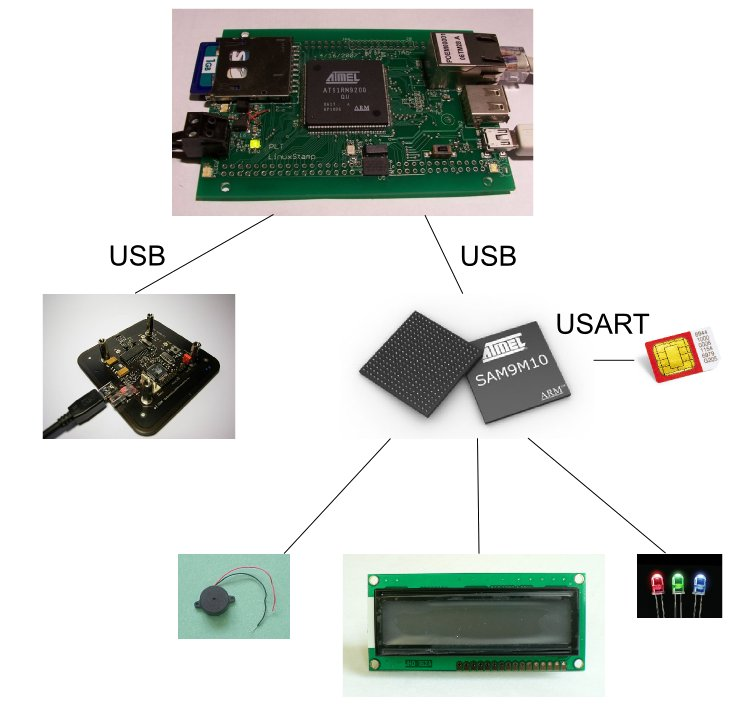
\includegraphics[scale=.25]{Imagenes/1.jpg} 
  \end{center}
  \caption{Solución posible 1}\label{Fig:HW} 
\end{figure}

Esta arquitectura tiene como ventaja el uso de la SBC que permite instalar un sistema operativo, reutilizar código ya implementado, posee varios puertos de E/S (I2C, USART, SPI, USB, GPIO, etc.), tiene gran capacidad de procesamiento, maneja memoria externa y brinda facilidad para realizar prototipos. Otra ventaja es el uso del microcontrolador que actúa como co-procesador, manejando el resto de los periféricos.

\item[2 -] SBC + OpenPCD + lector de tarjetas de contacto + display + buzzer + leds
El OpenPCD se conecta por USB a la SBC. La SBC maneja el resto de los dispositivos (lector de tarjetas de contacto, display, buzzer y leds) a través de sus interfaces nativas.

\begin{figure}[H]
\centering
  \begin{center}
  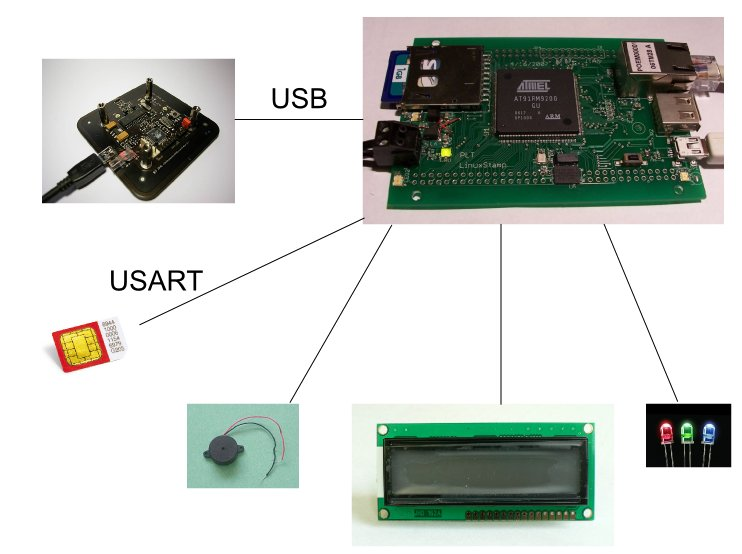
\includegraphics[scale=.25]{Imagenes/2.jpg} 
  \end{center}
  \caption{Solución posible 2}\label{Fig:HW} 
\end{figure}

\newpage

\item[3 -] SBC + lectores de tarjetas + display + buzzer + leds
Todos los periféricos (lectores de tarjetas, display, buzzer y leds) se conectan a la SBC a través de sus interfaces nativas, también el integrado CL RC632 de Philips que maneja la comunicación con las tarjetas sin contacto. Se diseña la antena para propagar RF.

\begin{figure}[H]
\centering
  \begin{center}
  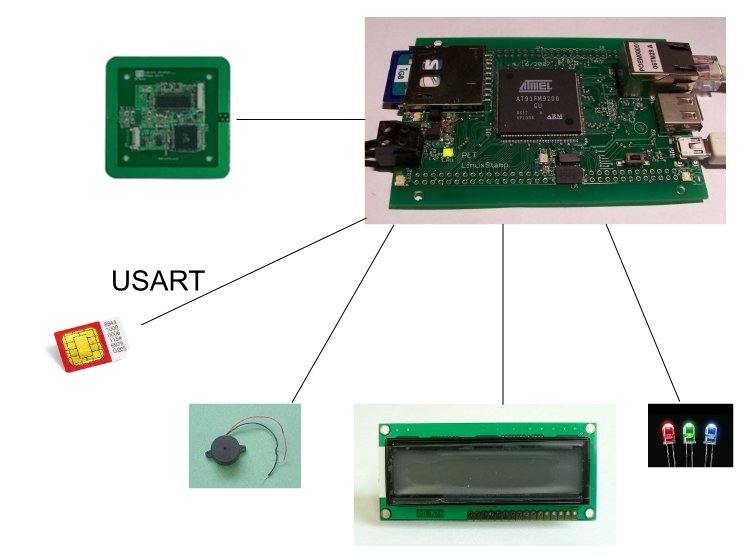
\includegraphics[scale=.25]{Imagenes/3.jpg} 
  \end{center}
  \caption{Solución posible 3}\label{Fig:HW} 
\end{figure}

\item[4 -] microcontrolador + lectores de tarjetas + display + buzzer + leds
Consta de un único PCB, que posee un microcontrolador como sistema central al cual se
conectan el resto de los dispositivos. Dicho PCB tiene incorporada la antena para la
propagación de RF. Se prevee el agregado de un modem 3G.

\begin{figure}[H]
\centering
  \begin{center}
  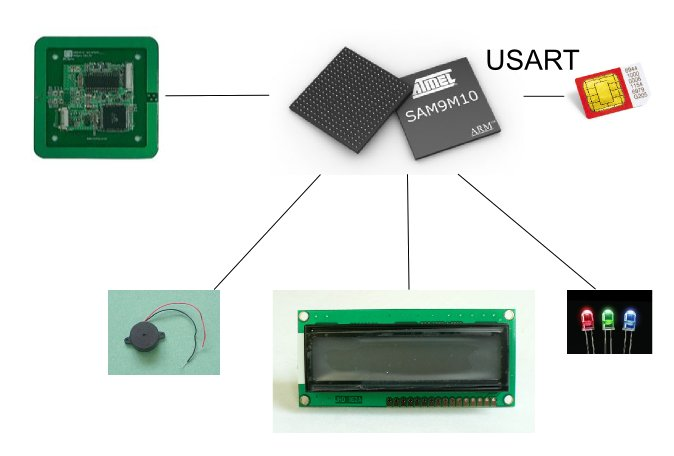
\includegraphics[scale=.25]{Imagenes/4.jpg} 
  \end{center}
  \caption{Solución posible 4}\label{Fig:HW} 
\end{figure}

\end{itemize}

\newpage
\section{Arquitectura seleccionada}
Luego de estudiar ventajas y desventajas de las arquitecturas planteadas, y discutirlo con los tutores, se eligieron dos de las posibilidades:

\begin{itemize}
\item SBC + OpenPCD + lector de tarjetas de contacto + display + buzzer + leds
\item SBC + lectores de tarjetas + display + buzzer + leds
\end{itemize}

\begin{figure}[H]
\centering
  \begin{center}
  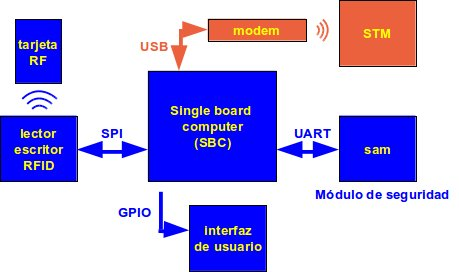
\includegraphics[scale=.5]{Imagenes/arq_def.jpg} 
  \end{center}
  \caption{Diagrama de bloques de la arquitectura seleccionada}\label{Fig:HW} 
\end{figure}

En principio se pensó en diseñar la primera opción como paso intermedio para testear el hardware diseñado, pensando en luego migrar a la segunda. De modo que, se migraría de la primer configuración a la segunda al diseñar e implementar un lector-escritor RFID que sustituya al OpenPCD.
Luego simplemente se diseñó la segunda, aunque se hicieron pruebas con el OpenPCD nunca se llegó a implementar por completo la primer configuración.

En una primera instancia se pretendía usar únicamente el dispositivo OpenPCD, ya que el mismo cuenta con un microcontrolador de la familia ARM, el AT91SAM7S128, una vez estudiado se llegó a la conclusión de que no permitía instalarle un kernel de Linux. Otra desventaja encontrada fue que sólo tiene un puerto I2C como forma de conectar periféricos.

Surge entonces la necesidad de usar una SBC como dispositivo capaz de correr un sistema operativo y ejecutar las aplicaciones necesarias para que el dispositivo cumpla con los requerimientos exigidos. El dispositivo OpenPCD pasaría entonces a cumplir la función de lector-escritor de tarjetas RFID, conectado a la SBC a través de su puerto USB, mientras que para el resto de los periféricos se diseñaría un pcb que fuera capaz de ser conectado a la SBC a través de sus interfaces nativas. Esta arquitectura fue descartada por el incremento en el costo del proyecto.

Fue necesario entonces descartar el uso del dispositivo OpenPCD y dar lugar a un diseño propio del lector-escritor de tarjetas RFID, usando para esto el integrado RC632 de Philips.

La última opción y la más ambiciosa, plantea el diseño completo de un pcb conteniendo un microcontrolador y memoria capaz de correr un sistema operativo, los lectores de tarjetas, tanto de contacto como RFID, un modem 3G y el resto de los periféricos (display, leds, buzzer). Esta opción fue dejada de lado por entender que excedería los plazos de tiempo del proyecto.


\section{Elecci\'on de hardware, m\'odulos}

\subsection{SBC}
En primera instancia se confeccionó una lista con posibles candidatas de SBC disponibles en el mercado internacional, teniendo en cuenta factores como: precio, puertos de E/S, memoria RAM, memoria Flash, puertos USB, Linux embebido, entre otros.
Se definieron una serie de requisitos mínimos necesarios para seleccionar de la lista la SBC que más se adecuara a la arquitectura definida.
Para la comunicación con el resto de los módulos será necesario: una interfaz UART para el módulo de seguridad (SAM); una interfaz SPI para el módulo lector-escritor RFID (RC632 de Philips); 20 GPIO para display, leds, buzzer, otros; 2 USB host, uno para la conexión de un módem 3G (intercambio de datos con un servidor central – STM) y otro para aplicaciones futuras. En cuanto a la memoria disponible debe ser de 32Mb de RAM y 8Mb de flash para el uso de un sistema operativo embebido. Es conveniente, pensando a futuro, que el procesador trabaje a una frecuencia no menor a 200MHz.
Dado el presupuesto estimado para el proyecto, el precio no debe superar los 150 dólares en origen.
Como requisito adicional se exigió que existiera un foro actualizado y soporte técnico que permita evacuar dudas.

%Aquí iría la tabla comparativa de las SBC, observar que allí no figura le Beagleboard


Aplicados los requisitos mínimos a la lista previamente confeccionada de SBC candidatas, optamos por dos: GESBC-9G20 y HAWKBOARD.
En cuanto a la primera opción, GESBC-9G20, los fabricantes no respondieron consultas, por tanto se descartó. Se optó entonces por la segunda opción, HAWKBOARD, puesto que respondieron a las consultas en tiempos razonables y se logró evacuar dudas desde el foro.


Finalmente, la SBC seleccionada para trabajar fue la BeagleBoard. Luego de recibir dos HAWKBOARD, ambas defectuosas, para intentar cumplir los plazos se optó por usar lo que se tenía a la mano (INCO) y justo cumplía los requisitos mínimos aunque se tuvo que diseñar otro módulo por problemas de voltajes.

\subsection{VLT - Conversor de Voltajes}
Este módulo no fue tenido en cuenta en la primera etapa del diseño de la arquitectura hardware, sino que surge como necesidad debido al cambio de SBC que nos vimos obligados a tomar. Como consecuencia de lo anterior vimos la ventaja de incorporar una placa que permite la conexión entre la SBC y el resto del hardware, el cual puede permanecer inalterado por más que no ocurra lo mismo con la SBC, ya que ésta puede cambiar de versión o dejar de fabricarse en un breve lapso de tiempo. El único elemento a cambiar sería entonces la placa VLT, que es más simple y barata de fabricar que las restantes partes.
La placa de circuito impreso VLT consta básicamente de dos conectores, uno de ellos permite la conexión con la Beagleboard y el otro la conexión con el restante hardware el cual se encuentra intergrado en un PCB llamdo SCUI. Ambos conectores no se encuentran directamente interconectados entre sí a través de pistas, pues para el caso particular de Beagleboard fue necesario incorporar conversores de tensión que permitieran el traslado del nivel de tensión desde 1,8 Volts que usa esta SBC, a las tensiones con las que operan los periféricos, ya sea 3,3 o 5 Volts.
El último elemento, no menos importante, es un regulador de tensión LDO que permite generar 3,3 Volts a partir de la fuente de tensión de 5 Volts de la propia Beagleboard.

\subsection{SCUI - Lector de tarjetas de contacto e Interfaz de Usuario}
La SAM es una tarjeta de contacto en la cual corre un sistema operativo y una máquina virtual de java, son también conocidas como java card y se utilizan en aplicaciones donde es necesario generar transacciones seguras. Este módulo permite encriptar datos y generar sesiones seguras con los servidores usados en la infraestructura del STM. Se precisa entonces un lector de tarjetas de contacto (SAM).


La interfaz de usuario se pensó como algo muy básico, que no genere confusiones al usuario durante una transacción y le indique que operaciones se están realizando sobre su tarjeta, como ser: consulta de saldo, incremento de saldo, etc. Para cumplir con lo anterior se optó por emplear un display LCD16x2, tres leds y un buzzer.
%Hasta aca es lo que teniamos en la documentacion para el hito1

\bigskip
\bigskip
\bigskip
El módulo SCUI puede dividirse en dos partes, una de ellas es un lector de tarjetas de contacto basadas en la norma ISO7816, y la otra es una simple interfaz para el usuario.
El lector de tarjetas de contacto(smart cards), está compuesto por un conversor full duplex a half duplex el cual se encuentra conectado a uno de los puertos UART de la SBC a través del módulo VLT, que se describió en el punto anterior. Este conversor permite la transmisión de datos directamente entre la tarjeta y la SBC, sin necesidad de intercalar un ASIC para el manejo de tarjetas del tipo ISO7816. Cuenta también con un oscilador para alimentar la entrada de reloj de las tarjetas. La entrada de control(OE) del oscilador operada desde la SBC permite poner la salida de reloj en tercer estado, cosa muy útil a la hora de cumplir con la secuencia de inicialización de las tarjetas descritas en el estandar. El lector permite operar con tarjetas clase A (alimentadas a 5 Volts) y clase B(alimentadas a 3,3 Volts) haciendo uso de un jumper que permite intercambiar la tensión de alimentación suministrada a la tarjeta. Se cuenta con un zócalo para insertar la tarjeta de contacto.
Por otra parte, la intefaz de usuario está compuesta por tres leds(verde, amarillo y rojo), buzzer y un display LCD16x2 donde son desplegados los mensajes que indican al usuario la operación que se efectúa sobre su tarjeta mifare.
El último elemento a describir aquí es un conector receptáculo 5x2(100mils) en el que se conecta el módulo lector/escritor RFID que opera con las tarjetas RFID mifare.

\subsection{Lector-Escritor RFID}
Si bien se descartó el uso del dispositivo OpenPCD, se toma como ejemplo para el
diseño del lector-escritor de tarjetas RF ya que el mismo se apega a las reglas de
diseño que establece el fabricante del integrado RC632.
Para detalles a tener en cuenta en la realización de una antena RF, ver Anexo I.



\section{Funcionamiento de m\'odulos}

\subsection{SBC}
La SBC contiene un microcontrolador y memoria que son capaces de correr un
sistema operativo, en este caso se usará la distribución Angstrom de Linux, la cual
está orientada a desarrollar sistemas embebidos. Sobre el sistema operativo se
instalan los módulos y librerías necesarias para hacer uso del hardware que contiene
la SBC. En nuestra aplicación usaremos uno de sus puertos SPI para la comunicación
con el lector-escritor de tarjetas RF, un puerto UART para la comunicación de datos
con el lector de tarjetas de contacto y varias salidas GPIO para el control de la
interfaz de usuario. Por último se usará uno de los puertos USB para agregar un
modem 3G que permita la conexión inalámbrica con un servidor para el intercambio
de datos.

\subsection{VLT - Conversor de Voltajes}
El corazón de esta placa son los integrados TXB0108[pdf] que permiten la interconexión de dispositivos que operan en distintos niveles de tensión. Básicamente el integrado está constituído por dos puertos, puerto A y puerto B cada uno de 8 bits. El puerto A opera con la tensión de 1,8 Volts que permite ser conectado a la Beagleboard, el puerto B opera con la tensión de 3,3 Volts en el caso que se encuentra conectado al IC RC632, y de 5 Volts para los restantes periféricos.
Cada I/O de un puerto es sensible a los flancos de subida o bajada, trasladando estos cambios a la I/O correspondiente del puerto opuesto. 
Este integrado posee también un entrada de control para poner los puertos en estado de alta impedancia.
Una ventaja es que no poseen entrada de control de dirección de flujo de datos, ahorrandonos pines de control que no tenemos disponibles en la Beagleboard.
En la figura debajo podemos observar como está constituído cada una de las entradas/salidas del integrado.
Otra pieza que compone esta placa es el regulador de tensión LDO implementado a partir del integrado LM1117[pdf], éste se usa para convertir la entrada de tensión de 5 Volts en una salida de tensión de 3,3 Volts y así poder alimentar el periférico correspondiente.

%pegar imágen de Arquitectura de una celda I/O del TXB0108, está en el pdf de la hoja de datos del txb0108

\subsection{SCUI - Lector de tarjetas de contacto e Interfaz de Usuario}

Las tarjetas de contacto que son empleadas para usos en telefonía celular (SIM) así
como también las empleadas en aplicaciones de seguridad (SAM) están formadas por
un microcontrolador y la comunicación con el mundo exterior la hacen a través de un
puerto UART half duplex. En nuestro diseño está contemplada la conversión de full
duplex a half duplex para poder interconectar la tarjeta de contacto a la SBC cuyo
puerto UART es full duplex.
Este tipo de tarjetas se operan mediante el uso de comandos APDU, donde la misma
responde a cada comando que es enviado desde el lado del terminal. La tarjeta sólo
envía una respuesta de manera espontánea, llamada ATR (Answer To Reset), para
indicar que ya está inicializada y lista para operar. En esta respuesta envía parámetros
al terminal como ser la tasa en bps a la que puede transferir los datos, etc. La tarjeta
nunca inicia la comunicación, actúa siempre como esclavo del terminal. La tarjeta
que emplearemos en esta aplicación es del tipo SAM, los comandos APDU para
operar con la tarjeta son específicos para la aplicación del STM. Mediante estos
comandos es posible abrir sesiones seguras con los servidores del STM, generar las
claves de lectura y escritura que luego son usadas para la comunicación con las
tarjetas RF, encriptar datos a ser enviados a los servidores, etc.
Las tarjetas de contacto (SAM) son suministradas por la Intendencia de Montevideo
y sólo sirven para operar con tarjetas RF de testing.


El display LCD16x2 está basado en un controlador de Hitachi, el HD44780, que
permite enviar comandos de control, o instrucciones de lectura-escritura a través de
su puerto de entrada paralelo. Una vez que es enviada la secuencia de inicialización
del display el mismo queda listo para operar, luego es posible enviar comandos para
ubicar el cursor en el lugar deseado o enviar los caracteres ASCII que formarán los
mensajes a ser desplegados para el usuario.
Los leds, al igual que el buzzer, tienen la función de complementar los mensajes
mostrados por el display. El led verde indica que la transacción se efectuó
correctamente, a la vez que se emite un pulso sonoro por el buzzer. El led rojo indica
que ocurrió un error, a la vez que el buzzer emite varios pulsos sonoros. El led
amarillo permanece encendido mientras no haya conexión con el servidor y por tanto
no se podrá operara con el dispositivo.

\bigskip
\bigskip
\bigskip

Lector de tarjetas de contacto ISO7816

Es un lector muy simple de implentar, su construcción se basa en un conversor full a half duplex construido a partir de un circuito transistorizado trabajando en zona de corte y saturación. Los transistores empleados son el NPN 2N3904[pdf] y el PNP 2N3906[pdf] los cuales fueron seleccionados en base a su rápida característica de conmutación que es del orden de alugnas decenas de nanosegundos. Dada la característica del circuito, es posible recibir el eco de la transmisión de datos generados por la SBC. 
Un elemento fundamental que compone el circuito del lector es el oscilador de frecuencia 3,579545 Mhz, este valor no es antojadizo sino que permite generar la base de tiempo adecuada para la transmisión de datos entre la tarjeta y la SBC. Otras frecuencias de reloj fueron empleadas, como ser 4 Mhz y 5 Mhz, con resultados inciertos en la recepción de los datos, aún cuando sería posible usar estos valores según la referencia [Smart Cards Handbook] para los parámetros obtenidos desde el ATR de la tarjeta. 
El circuito cuenta también con protección de descarga ESDA6V1W5[pdf] para los contactos de la smart card.


Interfaz de usuario

El elemento a destacar es un display LCD16x2 que basa su funcionamiento en el controlador Hitachi HD44780[pdf]. La transferencia de datos hacia el display se hace a través de un puerto con 4/8 bits de datos y 3 bits de control. Debido a no contar con la cantidad de pines disponibles en la Beagleboard para operar en el modo de 8 bits, se empleó en su lugar el modo 4 bits del display. El bit de control RS indica si el byte a enviar por el puerto de datos es una palabra de control o un caracter ASCII a ser almacenado en la memoria interna. El bit R/W por su parte indica si se efectuará una lectura o una escritura de la memoria interna del display. Por último en el bit E se indica mediante flanco de bajada que se ejecute la operación indicada con los anteriores dos bits de control, previo a este flanco la señal en el puerto de datos deben permanecer fijas.
El display cuenta también con una entrada para calibrar el contraste del LCD, la calibración se realiza a partir de un divisor resistivo implementado con resistencias y un preset.
El backlight del display es accionado desde uno de los pines de la SBC a partir de un circuito transistorizado que opera en zona de corte/saturación.
Los restantes elementos que componene la interfaz de usuario son leds y buzzer que son accionados directamente desde los pines del puerto de expansión de la SBC.

\subsection{Lector-Escritor RFID}
Este lector está compuesto entre otras cosas por el integrado RC632 que es capaz de
generar las señales que serán transmitidas hacia la antena RF. Si bien las tarjetas RF
usan un canal de transmisión diferente al que usan las tarjetas de contacto, el
principio de funcionamiento es el mismo. Cuentan con un microcontrolador y
responden a comandos APDU de la misma forma que las tarjetas de contacto. Los
comandos APDU serán enviados al integrado para ser convertidos en señales
analógicas que serán propagadas por la antena. La tarjeta que esté próxima al campo
magnético generado por la antena, será energizada por el mismo acorde a los
principios de la ley de Faraday. A esto se le llama acoplamiento entre antena y tarjeta.
Las tarjetas Mifare 1K cuentan con una estructura de memoria EEPROM de 1Kbytes
que se encuentra dividida en 16 sectores y a su vez cada sector dividido en 4 bloques.
En el cuarto bloque de cada sector se encuentran las claves de lectura-escritura de
dicho sector y las condiciones de acceso, estas claves no pueden ser leídas
directamente.
Cuando se envía un comando APDU a la tarjeta, por ejemplo para la lectura de un
bloque, previamente es necesario autenticarse con el sector al cual pertenece ese
bloque. Para autenticarnos debemos conocer la clave de lectura-escritura del sector,
esta clave la genera el módulo SAM a partir del identificador ID que caracteriza a
la tarjeta RF de forma única.
Las tarjetas RF que son usadas en este proyecto son suministradas por la Intendencia
de Montevideo y son tarjetas de testing, no pudiendo ser usadas en los ómnibus de
transporte de pasajeros.
